\section{Unseen-Participant Forecasting and the Limits of Simple Personalization}
\label{sec:forecasting_personalization}

\subsection{Motivation and research questions}

A glucose forecasting system intended for deployment must generalize beyond the
participants used during model training. A temporal holdout in which earlier
observations from the same participant are available during training measures
forecasting at future timestamps for a known individual. In contrast, a
participant-held-out evaluation tests whether the model can forecast a new
individual whose glucose trajectory was never observed during training.

This section investigates four related questions:

\begin{enumerate}
    \item How well did the original SSM-CGM architecture generalize to unseen
    AI-READI participants?
    \item Did the redesigned SSM-CGM Stream pipeline reduce the
    participant-held-out generalization error?
    \item Was the apparent improvement associated with longer nominal warm-up
    periods evidence of online personalization?
    \item Could a simple participant-specific bias correction improve later
    forecasts?
\end{enumerate}

The initial working hypothesis was that a global forecasting model would
require a dedicated adaptation phase for every new participant. The experiments
instead showed that the principal improvement came from the redesigned global
streaming pipeline. The subsequent warm-up and correction analyses did not
provide evidence that a constant participant-specific offset improved
future-anchor forecasting.

\subsection{Participant-held-out forecasting protocol}
\label{subsec:participant_held_out_protocol}

Participants were assigned to training, validation, and test sets using a
stratified participant-level split. No participant appeared in more than one
split:

\begin{equation}
\mathcal{P}_{\mathrm{train}}
\cap
\mathcal{P}_{\mathrm{validation}}
=
\mathcal{P}_{\mathrm{train}}
\cap
\mathcal{P}_{\mathrm{test}}
=
\mathcal{P}_{\mathrm{validation}}
\cap
\mathcal{P}_{\mathrm{test}}
=
\varnothing.
\end{equation}

The split was stratified using the AI-READI study groups: healthy,
prediabetes managed through lifestyle, type 2 diabetes managed without
insulin, and insulin-dependent type 2 diabetes. Normalization statistics and
target scales were estimated from the training participants only.

Each continuous participant segment was processed as an independent stream.
Forecast windows and recurrent states were not allowed to cross participant or
segment boundaries. At every 5-minute anchor $t$, the model emitted a
12-step forecast covering the next 60 minutes:

\begin{equation}
\hat{\mathbf{y}}_{i,t}
=
\left[
\hat{y}_{i,t+5},
\hat{y}_{i,t+10},
\ldots,
\hat{y}_{i,t+60}
\right].
\end{equation}

The deployable forecast-only evaluation used the observed history, static
clinical information, and known calendar information. It did not reveal future
wearable measurements or factual future actions to the decoder.

The principal metrics were mean absolute error, root mean squared error, and
forecast bias:

\begin{align}
\mathrm{MAE}
&=
\frac{1}{NH}
\sum_{i,t,h}
\left|
y_{i,t+h}-\hat{y}_{i,t+h}
\right|,
\\
\mathrm{RMSE}
&=
\sqrt{
\frac{1}{NH}
\sum_{i,t,h}
\left(
y_{i,t+h}-\hat{y}_{i,t+h}
\right)^2
},
\\
\mathrm{Bias}
&=
\frac{1}{NH}
\sum_{i,t,h}
\left(
\hat{y}_{i,t+h}-y_{i,t+h}
\right).
\end{align}

Negative bias indicates systematic underprediction. Because the model emits
the $0.1$, $0.5$, and $0.9$ quantiles, calibration was also assessed using the
empirical coverage of the nominal 80\% prediction interval.

Participant-level metrics were calculated before subgroup aggregation so that
participants with longer recordings did not dominate the subgroup estimates.
Where paired participant-bootstrap intervals were available, they were used for
inferential conclusions. Comparisons without such intervals are interpreted
descriptively and are not treated as statistically confirmed rankings.

\subsection{From the original SSM-CGM model to SSM-CGM Stream}
\label{subsec:historical_forecasting_progression}

The original Experiment C was the first SSM-CGM configuration evaluated using
a participant-disjoint split. Its global model achieved an MAE of
26.68~mg/dL and a bias of $-20.82$~mg/dL on unseen test participants. This
large negative bias indicated systematic underprediction rather than only
random forecast error.

The older pipeline also included a 48-hour adaptation procedure. After this
adaptation, MAE decreased to 21.21~mg/dL. Although the adaptation partially
reduced the initial generalization failure, the remaining error was still
large.

SSM-CGM Stream was subsequently introduced as a redesigned forecasting
pipeline. Its main changes included stateful segment-safe streaming,
static-profile initialization, FiLM conditioning, train-only scaling, and a
residual-current target representation:

\begin{equation}
\hat{y}_{t+h}
=
G_t+s_h\hat{r}_{t+h},
\end{equation}

where $G_t$ is the current observed glucose, $s_h$ is a horizon-specific scale
estimated on the training data, and $\hat{r}_{t+h}$ is the predicted normalized
change from the current glucose anchor.

The current Stream model achieved an MAE of 10.02~mg/dL and a bias of
$-1.446$~mg/dL. Table~\ref{tab:historical_forecasting_progression}
summarizes the historical progression.

\begin{table}[H]
\centering
\caption{Historical progression of participant-held-out forecasting. The
comparison describes the evolution of the complete forecasting pipeline and is
not a controlled component ablation.}
\label{tab:historical_forecasting_progression}
\begin{tabular}{lccc}
\toprule
Pipeline & Participant correction & MAE (mg/dL) & Bias (mg/dL) \\
\midrule
Old SSM-CGM global forecast
    & None
    & 26.68
    & $-20.82$ \\
Old SSM-CGM after adaptation
    & 48 h
    & 21.21
    & Not available in saved summary \\
SSM-CGM Stream
    & None in headline evaluation
    & 10.02
    & $-1.446$ \\
\bottomrule
\end{tabular}
\end{table}

Figure~\ref{fig:forecasting_progression} shows the corresponding progression in
MAE and bias.

\begin{figure}[H]
    \centering
    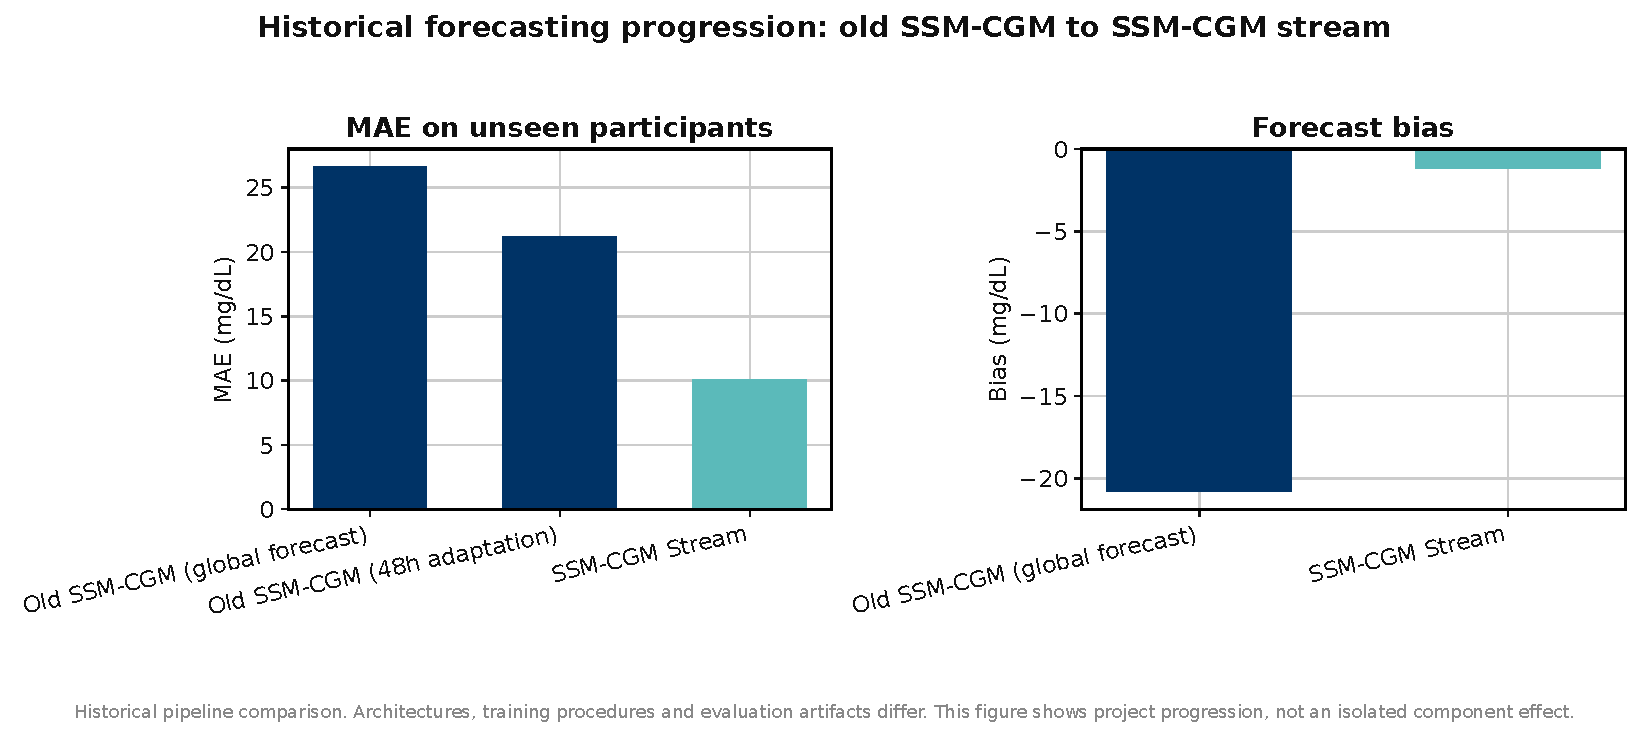
\includegraphics[width=\textwidth]
    {figures/forecasting_story/fig_forecasting_progression.pdf}
    \caption{Historical forecasting progression from the original
    participant-held-out SSM-CGM Experiment C to SSM-CGM Stream. The older
    model exhibited high error and severe systematic underprediction. The
    current Stream pipeline substantially reduces both quantities. Because the
    architectures, target transforms, preprocessing, training procedures, and
    saved evaluation artifacts differ, this figure demonstrates project
    progression rather than the isolated effect of one architectural
    component.}
    \label{fig:forecasting_progression}
\end{figure}

Relative to the original global Experiment C result, the Stream pipeline
reduced MAE by 16.66~mg/dL and reduced the magnitude of the negative bias by
approximately 19.37~mg/dL. The main conclusion is therefore that the complete
redesign substantially improved generalization to unseen participants. It is
not possible to attribute the entire gain to one change from this historical
comparison alone.

\subsection{Current SSM-CGM Stream forecasting performance}
\label{subsec:stream_headline_performance}

The deployable forecast-only model achieved an overall MAE of 10.02~mg/dL,
an RMSE of 15.95~mg/dL, and a bias of $-1.446$~mg/dL on the held-out test
participants. The nominal 80\% interval achieved a coverage of 79.3\%, close to
its intended population-level coverage.

The terminal 60-minute MAE was 14.43~mg/dL. This value is reported separately
from the multi-horizon average because the latter combines substantially easier
near-term predictions with the more difficult final forecast steps.

\begin{table}[H]
\centering
\caption{Headline forecast-only performance of SSM-CGM Stream on
participant-held-out test data.}
\label{tab:stream_headline_metrics}
\begin{tabular}{lc}
\toprule
Metric & Value \\
\midrule
Multi-horizon MAE & 10.02 mg/dL \\
RMSE & 15.95 mg/dL \\
Bias & $-1.446$ mg/dL \\
Terminal 60-minute MAE & 14.43 mg/dL \\
Nominal 80\% interval coverage & 79.3\% \\
True TIR 70--180 mg/dL & 89.7\% \\
Predicted TIR 70--180 mg/dL & 91.6\% \\
TIR gap & $+1.86$ percentage points \\
90th percentile absolute error & 24.25 mg/dL \\
95th percentile absolute error & 34.05 mg/dL \\
99th percentile absolute error & 59.69 mg/dL \\
\bottomrule
\end{tabular}
\end{table}

The near-nominal interval coverage indicates reasonable population-level
uncertainty calibration. However, the predicted TIR exceeds the observed TIR,
showing a modest tendency to place glucose inside the target range more often
than occurred in the data.

\subsection{Anchor-selection audit of the nominal warm-up analysis}
\label{subsec:warmup_anchor_selection_audit}

The original evaluation reported forecasting metrics after nominal warm-up
periods of 0, 6, 12, 24, and 48 hours. The unmatched sweep appeared to show a
progressive decrease in MAE:

\begin{equation}
10.07
\rightarrow
10.06
\rightarrow
10.02
\rightarrow
9.90
\rightarrow
9.76~\mathrm{mg/dL}.
\end{equation}

However, increasing the nominal warm-up duration progressively removed early
forecast anchors. The number of scored horizon-level predictions decreased
from approximately 9.31 million at 0 hours to 4.92 million at 48 hours.
Consequently, each point represented a different subset of participants,
segments, and timestamps.

\begin{table}[H]
\centering
\caption{Original unmatched nominal warm-up sweep. Because the evaluated rows
change with warm-up duration, this table is descriptive and does not establish
an adaptation effect.}
\label{tab:unmatched_warmup}
\begin{tabular}{rrrrr}
\toprule
Nominal warm-up & Scored horizon predictions & MAE & Bias & Coverage \\
\midrule
0 h  & 9,306,780 & 10.07 & $-1.16$ & 79.2\% \\
6 h  & 8,758,200 & 10.06 & $-1.24$ & 79.3\% \\
12 h & 8,209,560 & 10.02 & $-1.28$ & 79.3\% \\
24 h & 7,112,280 & 9.90  & $-1.40$ & 79.4\% \\
48 h & 4,917,720 & 9.76  & $-1.56$ & 79.5\% \\
\bottomrule
\end{tabular}
\end{table}

A common-anchor re-scoring analysis then restricted every nominal warm-up row
to the same 81,962 forecast anchors from 221 participants. Each anchor
contributed 12 forecast horizons, corresponding to 983,544 horizon-level
predictions. Under this common scoring set, MAE, bias, and interval coverage
were identical across all five nominal warm-up values.

\begin{table}[H]
\centering
\caption{Common-anchor re-scoring of the nominal warm-up analysis. The same
81,962 forecast anchors from 221 participants are used in every row.}
\label{tab:matched_warmup}
\begin{tabular}{rrrrrr}
\toprule
Nominal warm-up & Forecast anchors & Participants & MAE & Bias & Coverage \\
\midrule
0 h  & 81,962 & 221 & 9.76 & $-1.57$ & 79.5\% \\
6 h  & 81,962 & 221 & 9.76 & $-1.57$ & 79.5\% \\
12 h & 81,962 & 221 & 9.76 & $-1.57$ & 79.5\% \\
24 h & 81,962 & 221 & 9.76 & $-1.57$ & 79.5\% \\
48 h & 81,962 & 221 & 9.76 & $-1.57$ & 79.5\% \\
\bottomrule
\end{tabular}
\end{table}

Figure~\ref{fig:warmup_audit} contrasts the original unmatched curve with the
common-anchor result.

\begin{figure}[H]
    \centering
    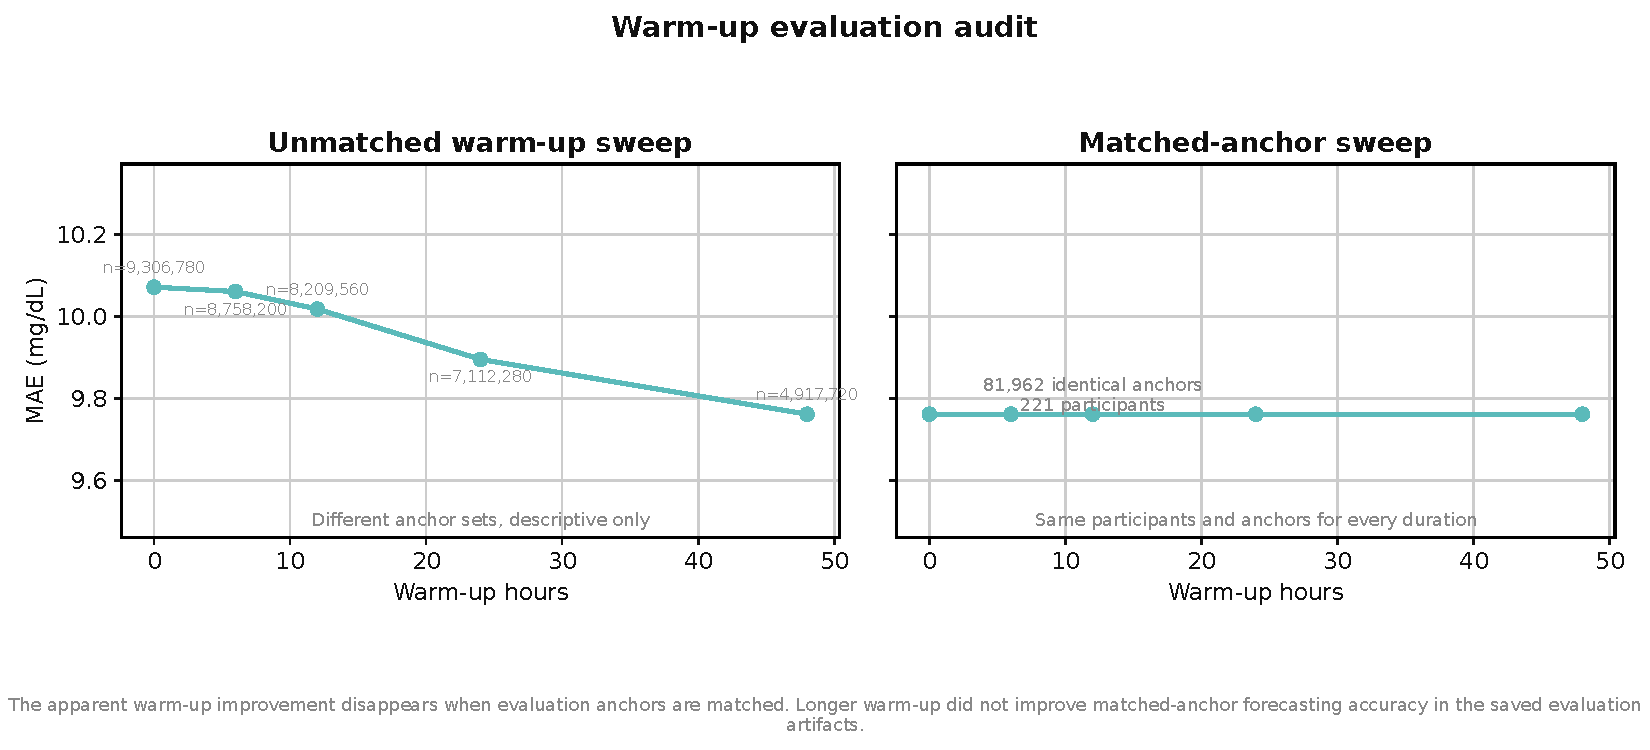
\includegraphics[width=\textwidth]
    {figures/forecasting_story/fig_warmup_audit.pdf}
    \caption{Anchor-selection audit of the nominal warm-up analysis. The
    unmatched sweep appears to improve because longer cutoffs remove early
    prediction anchors. When the same 81,962 anchors from 221 participants are
    re-scored, the metrics are identical across nominal warm-up values. The
    matched predictions originate from the same continuously propagated
    streaming state; therefore, the analysis diagnoses anchor-selection bias
    but does not constitute a controlled state-reset experiment.}
    \label{fig:warmup_audit}
\end{figure}

The correct interpretation is that the apparent improvement in the original
sweep was explained by changes in the evaluated anchor composition. The
common-anchor analysis does not directly manipulate how much history is used
to construct the recurrent state. At a given common anchor, the model had
processed the same preceding stream, regardless of the nominal warm-up label
assigned during scoring.

Therefore, these results should not be used to claim that the recurrent state
does not use historical information or that the model has definitively been
shown to be warm-up-free. They establish the narrower result that the original
warm-up curve was not evidence of personalization.

\subsection{Bias-based participant correction}
\label{subsec:bias_personalization}

The next experiment tested an explicit low-capacity form of participant
adaptation. The base SSM-CGM Stream model remained frozen. For participant
$i$ and forecast horizon $h$, a correction was estimated from residuals
observed in an adaptation interval $\mathcal{A}_i$:

\begin{equation}
b_{i,h}
=
\frac{1}{|\mathcal{A}_i|}
\sum_{t\in\mathcal{A}_i}
\left(
y_{i,t+h}
-
\hat{y}_{i,t+h}
\right).
\end{equation}

The corrected forecast was:

\begin{equation}
\hat{y}^{\,\mathrm{corrected}}_{i,t+h}
=
\hat{y}_{i,t+h}
+
b_{i,h}.
\end{equation}

This method tests whether the participant's mean past residual is sufficiently
stable to correct later predictions.

Four modes were compared:

\begin{enumerate}
    \item the raw frozen Stream forecast;
    \item an offset-corrected forecast;
    \item the existing participant-personalized forecast;
    \item the personalized forecast followed by an additional offset
    correction.
\end{enumerate}

\begin{table}[H]
\centering
\caption{Forecast accuracy and bias after participant correction. Lower MAE is
better. Bias is defined as prediction minus observation.}
\label{tab:personalization_bias}
\begin{tabular}{lcc}
\toprule
Mode & MAE (mg/dL) & Bias (mg/dL) \\
\midrule
Raw Stream forecast & \textbf{10.02} & $-1.446$ \\
Offset-corrected & 10.16 & approximately $0$ \\
Personalized & 10.52 & $-1.142$ \\
Personalized + offset-corrected & 10.61 & $+0.305$ \\
\bottomrule
\end{tabular}
\end{table}

Figure~\ref{fig:personalization_audit} shows the corresponding MAE and bias
results.

\begin{figure}[H]
    \centering
    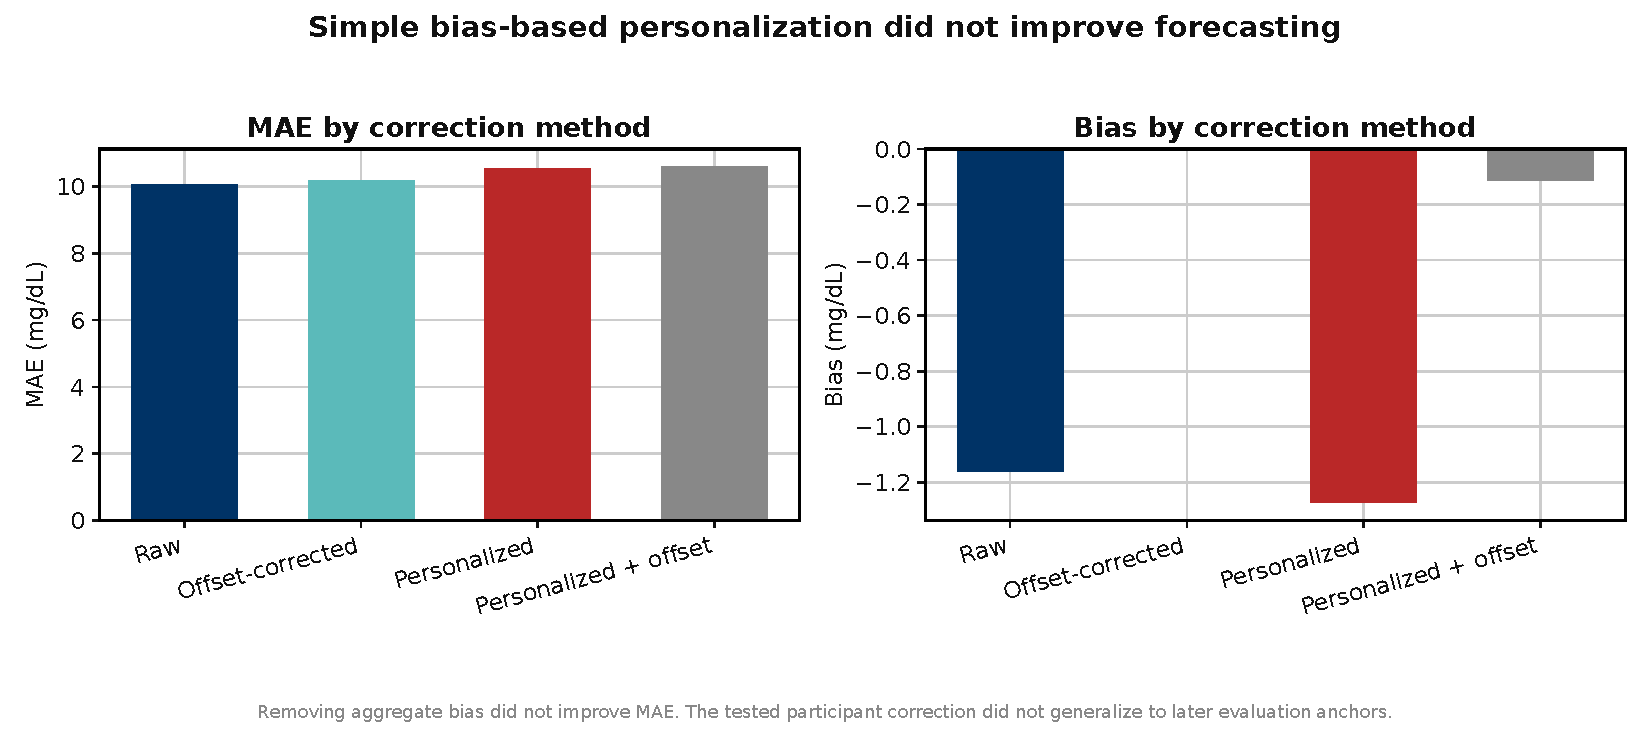
\includegraphics[width=\textwidth]
    {figures/forecasting_story/fig_personalization_audit.pdf}
    \caption{Audit of simple bias-based personalization. Offset correction
    removes the aggregate negative bias but increases MAE. Both personalized
    variants also perform worse than the uncorrected Stream forecast. Reducing
    population-level bias therefore did not translate into more accurate
    future-anchor predictions.}
    \label{fig:personalization_audit}
\end{figure}

The result demonstrates that:

\begin{equation}
\mathrm{Bias}\approx0
\quad\not\Rightarrow\quad
\mathrm{MAE}\text{ decreases}.
\end{equation}

A participant may exhibit positive forecast errors in one physiological regime
and negative errors in another. A single correction estimated from their
average past residual can therefore shift already-correct forecasts in the
wrong direction.

The remaining error is not well described as a stable participant-specific
vertical offset. It is more plausibly associated with changing glucose
direction, glycemic state, time of day, meals, activity, sleep, treatment, or
other unobserved events.

This result is method-specific. It shows that the tested bias-based correction
did not improve forecasting. It does not establish that every possible form of
personalization is ineffective.

\subsection{Convergence-based selection of the adaptation window}
\label{subsec:convergence_adaptation}

A fixed adaptation window may be unnecessarily long for some participants and
insufficient for others. A convergence-based procedure was therefore used to
estimate when the participant-specific horizon corrections stopped changing.

The correction was refitted in 6-hour increments up to a maximum of 48 hours.
Let:

\begin{equation}
\mathbf{b}^{(W)}_i
=
\left[
b^{(W)}_{i,5},
\ldots,
b^{(W)}_{i,60}
\right]
\end{equation}

denote the vector of horizon-specific corrections estimated after $W$ hours.
A participant was considered converged when:

\begin{equation}
\max_h
\left|
b^{(W)}_{i,h}
-
b^{(W-6)}_{i,h}
\right|
<
3~\mathrm{mg/dL}
\end{equation}

for three consecutive 6-hour increments.

The analysis included 287 participants. Of these, 194 converged within 48
hours and 93 did not. The median convergence time was 30 hours, with the 10th
and 90th percentiles at 24 and 36 hours.

\begin{table}[H]
\centering
\caption{Summary of the convergence-based adaptation-window analysis.}
\label{tab:convergence_summary}
\begin{tabular}{lc}
\toprule
Quantity & Result \\
\midrule
Total participants & 287 \\
Converged within 48 h & 194 \\
Did not converge & 93 \\
Convergence rate & 67.6\% \\
Median convergence time & 30 h \\
10th percentile & 24 h \\
90th percentile & 36 h \\
\bottomrule
\end{tabular}
\end{table}

Forecast improvement for participant $i$ was defined as:

\begin{equation}
\Delta\mathrm{MAE}_i
=
\mathrm{MAE}_{i,\mathrm{raw}}
-
\mathrm{MAE}_{i,\mathrm{corrected}}.
\end{equation}

Positive values indicate that the correction improved forecasting, while
negative values indicate degradation.

\begin{table}[H]
\centering
\caption{Convergence status and future-anchor forecast outcome.}
\label{tab:convergence_outcome}
\begin{tabular}{lcc}
\toprule
Outcome & Participants & Percentage \\
\midrule
Converged and improved & 76 & 26.5\% \\
Converged but worsened & 118 & 41.1\% \\
Did not converge & 93 & 32.4\% \\
\bottomrule
\end{tabular}
\end{table}

Among the 194 converged participants, 118, or 60.8\%, were worsened by the
correction. Only 39.2\% of converged participants improved.

The mean improvement was negative for every adaptation-window strategy.

\begin{table}[H]
\centering
\caption{Mean MAE improvement by adaptation-window strategy. Positive values
indicate improvement; negative values indicate degradation.}
\label{tab:adaptation_strategy_improvement}
\begin{tabular}{lc}
\toprule
Strategy & Mean MAE improvement (mg/dL) \\
\midrule
Fixed 24 h & $-0.191$ \\
Fixed 48 h & $-0.168$ \\
Convergence-based & $-0.148$ \\
\bottomrule
\end{tabular}
\end{table}

Figure~\ref{fig:convergence_outcome} separates numerical convergence from
forecasting benefit.

\begin{figure}[H]
    \centering
    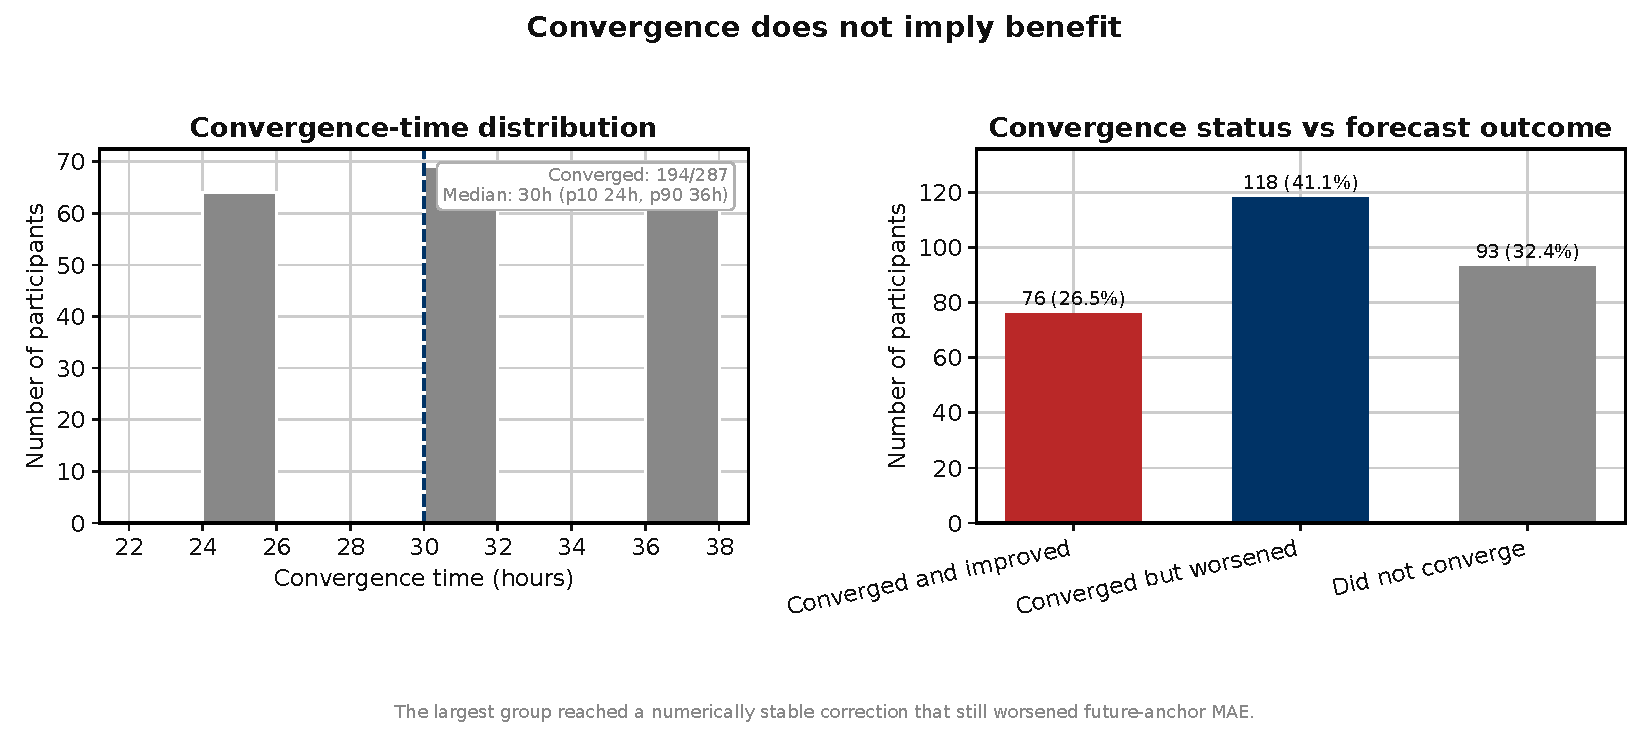
\includegraphics[width=\textwidth]
    {figures/forecasting_story/fig_convergence_outcome.pdf}
    \caption{Convergence does not imply forecasting benefit. Most converged
    corrections stabilized between 24 and 36 hours. Nevertheless, the largest
    group consisted of participants whose correction converged but worsened
    future-anchor MAE. Numerical stability of the fitted correction is therefore
    not evidence that the correction generalizes to later data.}
    \label{fig:convergence_outcome}
\end{figure}

The convergence-based strategy showed the smallest numerical mean degradation,
$-0.148$~mg/dL compared with $-0.191$ and $-0.168$~mg/dL. However, this
ordering has not been tested using paired participant-bootstrap confidence
intervals and should be read descriptively rather than as a confirmed ranking.
All three strategies failed to improve average forecasting accuracy.

Convergence answers whether the fitted correction stopped moving. It does not
answer whether the correction predicts future residuals. A stable estimate of
error in the adaptation interval may fail when the subsequent evaluation
interval contains different meals, activity, sleep, treatment, or glycemic
states.

\subsection{Forecasting heterogeneity across clinical subgroups}
\label{subsec:forecasting_subgroups}

The overall MAE hides substantial heterogeneity across participants.
Participant-level MAE was therefore calculated first and then aggregated within
clinical subgroups.

\subsubsection{Study group and HbA1c}

Mean participant MAE increased from 8.97~mg/dL in healthy participants to
12.64~mg/dL in the insulin-dependent study group. A similar gradient was
observed across HbA1c quartiles, from 8.83~mg/dL in the lowest quartile to
12.63~mg/dL in the highest quartile.

\begin{table}[H]
\centering
\caption{Participant-level forecasting performance by AI-READI study group.}
\label{tab:study_group_forecasting}
\begin{tabular}{lrrr}
\toprule
Study group & $N$ & Mean MAE & Median MAE \\
\midrule
Healthy & 78 & 8.97 & 8.72 \\
Prediabetes & 56 & 9.42 & 9.16 \\
T2D oral/non-insulin & 64 & 11.31 & 11.26 \\
T2D insulin-dependent & 23 & 12.64 & 12.64 \\
\bottomrule
\end{tabular}
\end{table}

\begin{table}[H]
\centering
\caption{Participant-level forecasting performance by baseline HbA1c quartile.}
\label{tab:hba1c_forecasting}
\begin{tabular}{lrrrr}
\toprule
Quartile & HbA1c range (\%) & $N$ & Mean MAE & Median MAE \\
\midrule
Q1 & 3.8--5.4 & 58 & 8.83 & 8.41 \\
Q2 & 5.4--5.8 & 60 & 9.06 & 8.79 \\
Q3 & 5.8--6.3 & 45 & 10.22 & 10.07 \\
Q4 & 6.3--12.5 & 54 & 12.63 & 12.23 \\
\bottomrule
\end{tabular}
\end{table}

The difference between the insulin-dependent and healthy groups was
3.67~mg/dL. The difference between the highest and lowest HbA1c quartiles was
3.80~mg/dL.

\subsubsection{Insulin-use metadata}

Participants with recorded insulin use had a mean participant MAE of
12.83~mg/dL, compared with 9.92~mg/dL among participants without recorded
insulin use.

\begin{table}[H]
\centering
\caption{Participant-level forecasting performance by insulin-use metadata.}
\label{tab:insulin_forecasting}
\begin{tabular}{lrr}
\toprule
Insulin metadata & $N$ & Mean MAE \\
\midrule
No recorded insulin use & 204 & 9.92 \\
Recorded insulin use & 17 & 12.83 \\
\bottomrule
\end{tabular}
\end{table}

The insulin-dependent study-group category and the medication-derived
\texttt{med\_insulin} flag are related but not equivalent definitions. Their
sample sizes differ because study-group classification and medication metadata
have different availability and inclusion rules.

\subsubsection{Clinical site}

Site-level mean participant MAE ranged from 9.78~mg/dL at UCSD to
10.55~mg/dL at UAB.

\begin{table}[H]
\centering
\caption{Participant-level forecasting performance by clinical site.}
\label{tab:site_forecasting}
\begin{tabular}{lrr}
\toprule
Clinical site & $N$ & Mean MAE \\
\midrule
UAB & 82 & 10.55 \\
UW & 85 & 9.98 \\
UCSD & 54 & 9.78 \\
\bottomrule
\end{tabular}
\end{table}

Figure~\ref{fig:stream_subgroups} presents the four subgroup views together.

\begin{figure}[H]
    \centering
    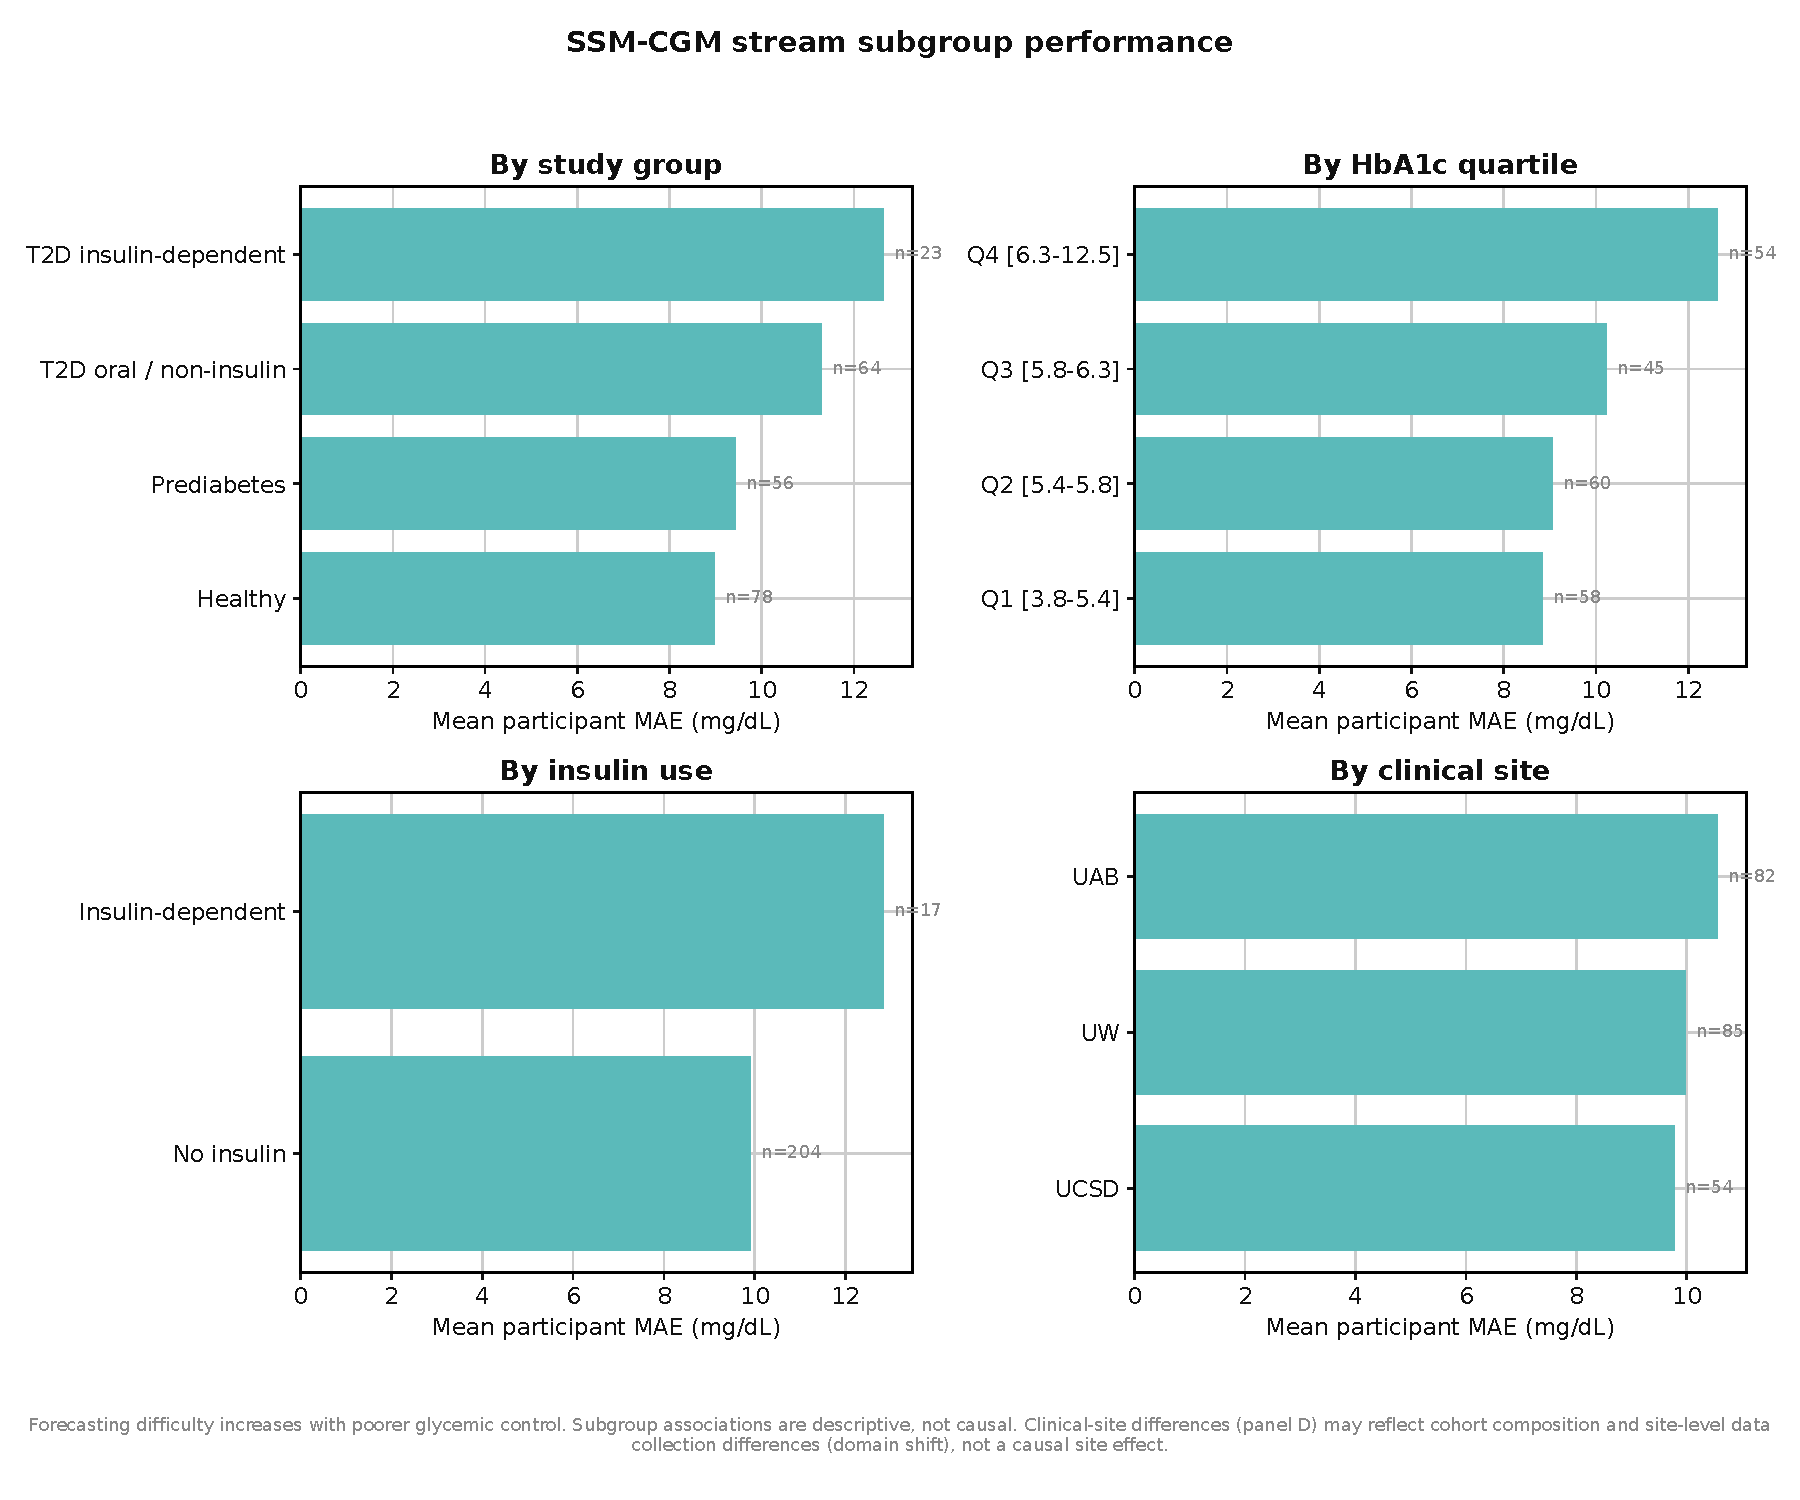
\includegraphics[width=\textwidth]
    {figures/forecasting_story/fig_stream_subgroups.pdf}
    \caption{Participant-level SSM-CGM Stream forecasting performance by study
    group, HbA1c quartile, insulin-use metadata, and clinical site. Forecasting
    error increases with more complex glycemic phenotypes and higher HbA1c.
    Clinical-site differences are smaller and may reflect cohort composition,
    acquisition conditions, missingness, or other domain-shift effects. The
    associations are descriptive and should not be interpreted causally.}
    \label{fig:stream_subgroups}
\end{figure}

The phenotype and HbA1c gradients were substantially larger than the site
gradient. The site range was only:

\begin{equation}
10.55-9.78
=
0.77~\mathrm{mg/dL},
\end{equation}

whereas the phenotype and HbA1c ranges were approximately 3.7--3.8~mg/dL.

Possible explanations for the higher error in insulin-dependent and
higher-HbA1c participants include greater glucose variability, more frequent
rapid excursions, more complex treatment-response dynamics, and unobserved
insulin or behavioral events. These interpretations remain hypotheses because
treatment status, HbA1c, glycemic variability, and study group are correlated.

\subsection{Published SSM-CGM and TFT results as contextual references}
\label{subsec:published_context}

The original SSM-CGM paper compared SSM-CGM with a Temporal Fusion
Transformer under a common within-participant temporal-holdout protocol
\cite{isaac2025ssmcgm}. TFT was selected as the principal
comparator after outperforming LightGBM, DeepAR, N-HiTS, and a Seq2Seq LSTM in
the paper's initial benchmarking.

Under that matched paper protocol, SSM-CGM consistently outperformed TFT at
12-, 24-, and 48-hour context lengths.

\begin{table}[H]
\centering
\caption{Published SSM-CGM and TFT performance under the original paper
protocol. Values are means with 95\% confidence intervals. These values are
contextual references and are not directly matched to the current
participant-held-out study.}
\label{tab:published_ssmcgm_tft}
\resizebox{\textwidth}{!}{
\begin{tabular}{llccc}
\toprule
Context & Model & Quantile loss & MAE (mg/dL) & RMSE (mg/dL) \\
\midrule
12 h
& SSM-CGM
& 3.87 (3.81--3.93)
& 5.97 (5.68--6.26)
& 7.17 (6.83--7.52) \\
12 h
& TFT
& 3.95 (3.89--4.02)
& 6.07 (5.76--6.37)
& 7.32 (6.96--7.69) \\
\midrule
24 h
& SSM-CGM
& 3.69 (3.63--3.75)
& 5.66 (5.39--5.93)
& 6.86 (6.53--7.19) \\
24 h
& TFT
& 3.92 (3.86--3.99)
& 6.06 (5.77--6.36)
& 7.28 (6.93--7.63) \\
\midrule
48 h
& SSM-CGM
& 3.52 (3.47--3.58)
& 5.40 (5.15--5.65)
& 6.56 (6.26--6.87) \\
48 h
& TFT
& 3.70 (3.64--3.76)
& 5.77 (5.50--6.03)
& 6.92 (6.61--7.24) \\
\bottomrule
\end{tabular}
}
\end{table}

Figure~\ref{fig:published_context} visually separates the current AI-READI
participant-held-out experiments from the published within-participant temporal
holdout.

\begin{figure}[H]
    \centering
    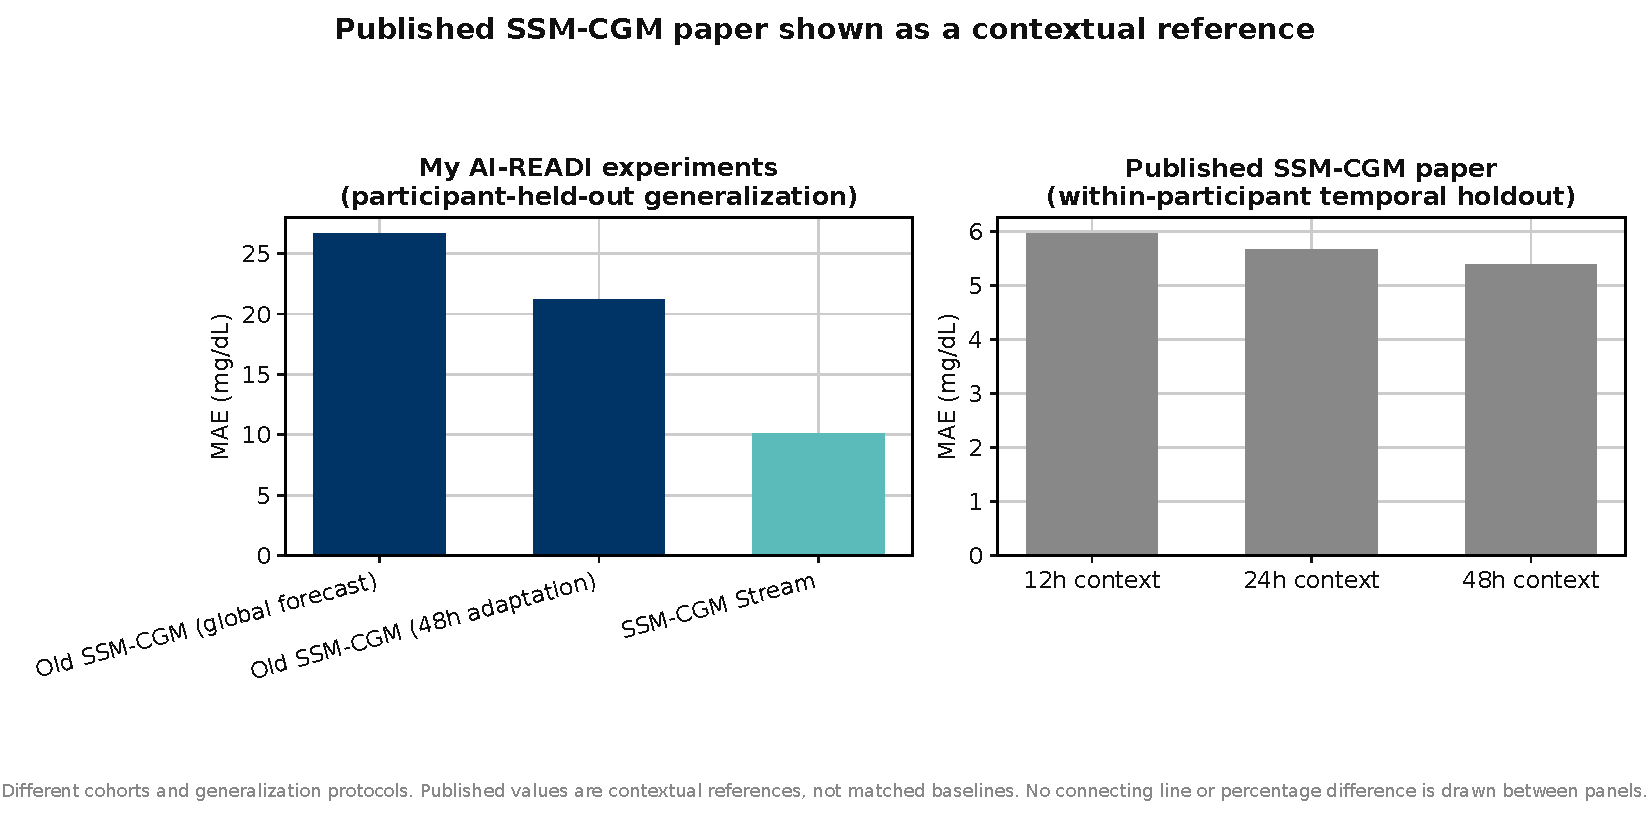
\includegraphics[width=\textwidth]
    {figures/forecasting_story/fig_published_contextual_reference.pdf}
    \caption{Published SSM-CGM results shown as contextual references. The
    current AI-READI experiments evaluate generalization to participants who
    were completely unseen during model training, whereas the published paper
    used a within-participant temporal holdout. The two panels therefore answer
    different generalization questions and should not be interpreted as a
    directly matched numerical comparison.}
    \label{fig:published_context}
\end{figure}

The lower MAEs reported in the paper do not imply that the published model
generalizes better to unseen participants. Conversely, the current results do
not demonstrate that SSM-CGM Stream outperforms TFT under the current protocol.
A fair architecture comparison would require training TFT on the same current
cohort, participant split, covariates, context, horizon, and forecast anchors.

\subsection{Discussion}
\label{subsec:forecasting_personalization_discussion}

\subsubsection{The main gain comes from the redesigned global pipeline}

The original participant-held-out Experiment C exposed a major generalization
failure. The global model had both high MAE and a large systematic negative
bias. A 48-hour adaptation phase partially reduced the error but did not solve
the problem.

SSM-CGM Stream substantially improved unseen-participant forecasting without
requiring the old adaptation procedure as part of the headline evaluation. The
historical progression is consistent with the combined effect of residual-current
anchoring, participant-safe streaming, static conditioning, improved
segmentation, and train-only normalization. Their individual contributions
cannot be isolated from the historical comparison alone.

\subsubsection{Reframing personalization}

The experiments distinguish several meanings of personalization:

\begin{table}[H]
\centering
\caption{Different forms of personalization considered in this work.}
\label{tab:personalization_definitions}
\begin{tabular}{p{0.25\textwidth}p{0.38\textwidth}p{0.28\textwidth}}
\toprule
Form & Mechanism & Current evidence \\
\midrule
Zero-shot participant conditioning
& Static clinical covariates initialize and modulate a global model.
& Present in SSM-CGM Stream. \\
Passive state accumulation
& The recurrent state carries observed participant history forward.
& The current cutoff audit does not directly manipulate state history. \\
Nominal warm-up scoring
& Early anchors are excluded before metrics are calculated.
& Apparent gain was explained by anchor selection. \\
Explicit bias correction
& Past residual means are applied to later forecasts.
& Reduced bias but worsened MAE. \\
Convergence-based correction
& Adaptation ends when fitted offsets stabilize.
& Stability did not imply future forecasting benefit. \\
\bottomrule
\end{tabular}
\end{table}

The results do not show that the model is non-personalized. Every prediction is
conditioned on a participant's static profile, current glucose, and accumulated
streaming state. What failed was the narrower assumption that future errors
could be corrected using one stable participant-specific offset estimated from
the first hours of data.

\subsubsection{Why a constant correction is insufficient}

A constant offset assumes:

\begin{equation}
e_{i,t,h}
\approx
b_{i,h}
\end{equation}

for future timestamps $t$. The observed degradation indicates that this
stationarity assumption is not generally valid. A more realistic residual model
would depend on the current state:

\begin{equation}
e_{i,t,h}
=
f_i
\left(
G_t,
\Delta G_t,
\text{time of day},
\text{meal state},
\text{exercise state},
\text{sleep},
\text{treatment context}
\right)
+
\epsilon_{i,t,h}.
\end{equation}

A participant may be overpredicted in one physiological regime and
underpredicted in another. Averaging these regimes into a single correction can
therefore degrade later forecasts.

\subsubsection{Implications for subsequent personalization work}

The remaining error is concentrated in participants with more complex glycemic
profiles and is unlikely to be resolved through a global vertical shift.
Subsequent personalization should therefore focus on dynamic response patterns,
including:

\begin{itemize}
    \item exercise and post-exercise glucose responses;
    \item rapid glucose rise and decline states;
    \item meal-associated excursions;
    \item sleep and overnight regulation;
    \item event-specific residual corrections;
    \item participant-specific counterfactual response curves.
\end{itemize}

Together with the meal-state audit, these findings define a consistent dataset
boundary: AI-READI supports rigorous participant-held-out forecasting and
model-behavior auditing, but fine-grained causal personalization remains limited
by the absence of prospectively observed meals, treatment timing, and behavioral
actions.

\subsection{Limitations}
\label{subsec:forecasting_personalization_limitations}

Several limitations qualify the conclusions of this section.

First, the old SSM-CGM and current SSM-CGM Stream results form a historical
pipeline comparison. They were not generated as a controlled architecture
ablation using identical checkpoints, preprocessing, and common forecast
anchors.

Second, the common-anchor warm-up analysis is a scoring audit rather than a
controlled state-reset experiment. It establishes that the original apparent
gain resulted from changing anchor composition, but it does not directly test
the effect of initializing the recurrent state at different times before the
same anchor.

Third, the participant correction is intentionally low capacity. Its failure
does not exclude nonlinear, event-specific, state-dependent, or
counterfactual-response personalization.

Fourth, the relative ordering of the 24-hour, 48-hour, and convergence-based
adaptation strategies remains descriptive because paired participant-bootstrap
confidence intervals were not used to compare the three mean degradations.

Fifth, subgroup analyses are observational and descriptive. Differences by
HbA1c, insulin use, study group, and clinical site may reflect overlapping
effects of treatment, glucose variability, cohort composition, missing
covariates, and acquisition conditions.

Finally, the published SSM-CGM and TFT results cannot be used as direct
benchmarks for the current participant-held-out model because they were
obtained using a different cohort construction and a within-participant temporal
holdout.

\subsection{Conclusion}
\label{subsec:forecasting_personalization_conclusion}

The original participant-held-out SSM-CGM experiment revealed a major
generalization failure, characterized by high MAE and severe systematic
underprediction for unseen participants. The redesigned SSM-CGM Stream
pipeline reduced MAE to 10.02~mg/dL and reduced bias to
$-1.446$~mg/dL while retaining near-nominal prediction-interval coverage.

The original nominal warm-up curve appeared to improve with longer warm-up,
but this pattern was explained by changes in the evaluated anchor set. Common
anchor re-scoring yielded identical metrics because the same continuously
propagated streaming predictions were scored in every nominal warm-up row.
This audit therefore identifies selection bias rather than proving a state
warm-up effect.

Explicit participant-level bias corrections removed aggregate bias but
increased MAE. Moreover, a correction could converge numerically while still
worsening future-anchor forecasts. The remaining error is therefore not well
represented by a stable participant-specific offset.

The central conclusion is:

\begin{quote}
SSM-CGM Stream substantially improves generalization to unseen participants
through the redesigned global forecasting pipeline. The tested nominal warm-up
and bias-based correction procedures do not provide evidence of additional
forecasting value. Future personalization should target dynamic,
event-dependent physiological responses rather than a constant participant
offset.
\end{quote}
